
\section{Introduction}

This chapter introduces WLDO, an automatic and end-to-end neural network which recovers the 3D pose and shape of dogs from monocular internet images. The large variation in shape between dog breeds, significant occlusion and low quality of internet images makes this a challenging problem. In addition, the dog cateogry is poorly represented by existing 3D morphable models. Despite the ubiquity of dogs in society (there are more than 63 million pet dogs in the US alone~\cite{appa20}), these factors have perhaps contributed to the lack of effective 3D reconstruction methods. 
This chapter demonstrates that the natural variation present in a 2D dataset is sufficient to learn a detailed 3D dog prior, which helps regularize parameter estimation. WLDO achieves this by adding additional limb scaling parameters to the morphable model, and including expectation maximization (EM) update steps into the network training loop. These contributions are shown experimentally to improve the quality of reconstruction. 
Presently, state of the art animal 3D reconstruction techniques incoporate per-image (or per-sequence as in \Cref{chap:cgas}) test time energy minimization procedures that prevent real-time application. Inspired by recent methods for human reconstruction ~\cite{kanazawa18end-to-end}, WLDO comprises an end-to-end convolutional neural network which directly regresses morphable model parameters with no subsequent energy minimization phase, achieving inference at approximately 10 frames per second. This is important for downstream tasks, such as animal monitoring systems, which rely on live data in order to alert experts to immediate causes for concern. 
The experimentation section is based on StanfordExtra, a new `in the wild' dataset of dog images, containing 120 breeds. The method presented achieves state of the art performance on this dataset, shows strong generalization characteristics to a new dataset, and outperforms model fitting approaches, even when they are given access to ground truth annotations at test time. 

%In comparison, the shape prior refinement process introduced here is applied only at training time and leads to improved shape reconstructions enabling high quality 3D dog predictions that make a subsequent refinement step optional. 

% WHY DOGS???
%A particular species of interest is the dog, however it is noticeable that existing work has not yet demonstrated effective 3D reconstruction of dogs over large test sets. We postulate that this is partially because dog breeds are remarkably dissimilar in shape and texture, presenting a challenge to the current state of the art.

% 

% The hope is to overcome limitations surrounding the practical application of such systems. For example, poor quality single-view shape reconstructions can lead to missed health and wellbeing insights, can lead to animal researchers are unable to analyse subtle differences in weight and body proportions which could otherwise lead to health and wellbeing insights. 

%A by-product of training, we generate a new parameterized model (including limb scaling) SMBLD which we release alongside our new annotation dataset StanfordExtra to the research community.

% Approach is weakly supervised deep network (i.e. we have no 3D training data)
% We adapt our 3D prior to be multi-modal
% We learn a 3D prior using a 2D image dataset
% Inspired by SPIN: this prior is learned using an optimization process during training time
% We adapt our 3D model using scale parameters
% Why dogs??


% 1) Improving model flexiblility with scale parameters
% 2) Implementation as a deep neural network to enable real-time
% 3) Learning a shape prior
% 4) Using EM in the loop to learn the 

% WORK IN some lit review stuff from the paper.

% \subsection{Animal datasets}

% To learn a representative 3D prior and enable quantitative comparison to existing state of the art methods, a large 2D animal dataset is required. Whereas existing methods typically evaluate on a few examples from multiple species, this work focuses solely on the dog category. Although focusing on a single category limits the overall shape diversity, the shape variation between breeds is significant and is more complex. Capturing subteleties between multiple Capturing these subtleties 

\subsection{Adding local parameters to the PCA shape space}


As discussed in \Cref{chap:relwork}, there is a long history of 3D reconstruction approaches which use morphable models to represent articulated subjects. Recently, the dominant paradigm is to factor the deformation space into a parameterization based on pose (which governs limb movements) and a global PCA shape space. While efficient and differentiable, even as early as the seminal paper of Blanz and Vetter \lazycite{blanz,vetter}, it was noted that these global representations poorly represent fine details (in their case, features such as the eyes and nose). Originally, this was tackled by manually segmenting the face into separate regions and learning separate PCA models per regions. While this does achieve higher fidelity modelling, it comes at the cost of a less compact shape space representation. Most closely related to the work in this chapter is the recent work of \lazycite{STAR}{STAR}, which is a drop in replacement for the original SMPL \lazycite{SMPL}{SMPL} human model. They note that the use of SMPL's global blend parameters result in the need for dense pose-corrective offsets, which relate every mesh vertex to every kinematic tree joint. This has the effect of capturing suprious long-range correlations between seemingly unrelated parts of the mesh. STAR improves over this with a local formulation, learning a set of mesh vertices which are influenced by each joint's movement. Another limitation of globally defined PCA spaces (which is of particular relevance to \Cref{chap:3dmulti}) is that it is difficult to relate uncertanties in a reconstructed shape to specific parts of the mesh. For example, since each body part is governed by multiple shape parameters, so are the uncertanties which makes it hard to reason about occluded parts.

These challenges are compounded in a low training data setting. The SMAL animal model is built from scans of 41 toy figurines, resulting a PCA space that captures correlations which coincidentally exist in the training corpus. Examples of this are shown in Figure XXX. This chapter demonstrates an approach for adding a few extra local shape parameters to the SMAL model, allowing the body part to scale independently to the rest of the mesh. These parameters help the model generalize to dogs outside of the 3D training samples, are an inexpensive addition to the generator function and produce better shape reconstructions for WLDO and a previous approach based on energy minimization. 

% TODO: Add an example of correlations. Can't control the tail!

\subsection{Automatic and real-time 3D dog reconstruction}

Early 3D reconstruction approaches in humans~\lazycite{examples}{examples} use an energy minimization framework which iteratively optimizes a 3D morphable model to match an input image or video sequence. These methods typically design an energy function that balances \emph{data terms} to encourage strong alignment between the 3D model and input image, and \emph{prior terms} which ensure realistic predictions. However, more recent works frame the reconstruction task as a direct regression from the input image to 3D model parameters and are typically implemented using convolutional neural networks. By learning from large datasets, deep learning approaches are now state of the art. Alongside fast test-time performance, methods learn accurate priors over the object category which lead to improved performance on images with occlusion and they do not fall into failure cases common to optimization techniques, generally caused by poor model initialization. However, a downside of deep learning methods is their reliance on large datasets. Apart from the input 3D morphable model (e.g. SMPL~\lazycite{SMPL}{SMPL}), typically required are large \emph{paired 3D datasets} and \emph{unpaired 2D datasets} containing images and 2D annotations. Paired 3D datasets help models learn an association between input image features and 3D shape and pose parameters. However, such datasets require specialized equipment to collect (e.g. motion capture) resulting in limited variety in captured scenes. To overcome this, unpaired 2D datasets typically containing 2D keypoint and/or silhouette annotations are used to help models generalize to ``in-the-wild'' scenarios. Occasionally, these methods are also evaluated in an `unpaired' setting, in which the paired datasets are ommited. Under these conditions, methods must overcome fundamental ambiguities to learn the 2D-to-3D mapping, or risk predicting 3D bodies with impossible joint angles or have implausible body weight distributions. Explicit 3D priors are often learned during training to ensure the predicted models lie on the manifold of plausible bodies. The ``unpaired'' training mode is of most relevance to this chapter's task of reconstructing 3D dogs, since paired 3D animal data is severely limited. Of concern, then, is how to design a suitable prior for the dog category. This is explored in depth in hte following sections.

Existing 3D animal reconstruction techniques are either entirely optimization based or incoporate optimization procedures as a part of the prediction pipeline. Notable exceptions include deep networks used to reconstruct unarticulated categories such as birds (e.g. CMU, UCMU) or the technique of Kulkarni et al.~\lazycite{Canonical Surface Mapping}{} which operates on articulated categories but does not recover shape characteristics. SMALST is perhaps the closest attempt to an end-to-end technique for articulated shape and pose recovery, although video sequences are required for training and a test-time optimization strategy is used to refine initial regressed parameters, preventing real time operation. Further, it can be argued that the zebra species tackled in this paper is more limited than the 120 dog breeds examined in this chapter. Inspired by these approaches and the recent end-to-end work in human mesh reconstruction, WLDO comprises a deep neural network that directly regresses 3D dog model parameters \emph{with no subsquent optimization phase} to enable real-time inference.

% Already written in the intro.
%This restricts the future practical use of such reconstruction systems, as future downstream tasks such as animal behaviour and health analysis systems would be restricted to processing pre-recorded video, rather than being able to immediately respond to causes for concern. 


\subsection{Learning a 3D animal prior}

% TODO: Incoporate this!
%Another method for improving the generalizability of the SMAL model is to improve the 3D shape prior. Such priors are typically used to ensure shape deformation remain within a realistic and anatomically plausible range. Due to the limited diversity of scans used to build the SMAL model, while the shape prior does enforce realism among deformations, it does not allow for a wide enough range to cover the set of dogs in our dataset.
 
While detailed 3D morphable models and associated priors are already available for humans~\lazycite{CMU}, the limited 3D training data for animals has made designing equivalent resources more difficult. The SMAL paper proposed an approach for building a morphable quadruped models from a few toy figurines rather than scans of real subjects (such as used for SMPL~\lazycite{SMPL}{SMPL}. Shape and pose priors were similarly collected by fitting the SMAL model to 2-3 artist animation sequences. Consequently, the SMAL model and priors are of relatively low fidelity and poorly represent some species, particularly dogs. Alongside the prevalence of challenging poses, occlusion and difficult environmental factors, overly restrictive animal priors have likely contributed to the lack of effective 3D reconstruction approaches for the dog category. \Cref{chap:cgas} has already demonstrated an example of this, in which synthetically data generated according to the SMAL prior was used to train a 2D joint predictor. While high quality results are shown on categories better represented by SMAL, the experimental section of this chapter shows the method generalizes poorly to some out-of-domain dog breeds. 

Some recent deep learning methods overcome this by forgoing data-driven 3D priors for the regression task altogether. SMALST is one such example; they supervise a deep network using 3D synthetic models generated using video sequences. Other techniques \lazycite{birds, dolphins}{} instead use smoothness terms, deformation constraints and symmetry constraints, although these are only effective when modelling unarticulated categories such as birds and dolphins. Of course, the quality of 3D morphable models, animal priors and potentially reconstruction results could be improved by collecting larger datasets of detailed 3D scans. However, collecting such a dataset would be expensive and time-consuming, either relying on scans of real animal subjects or contracting talented 3D graphics artists to build hundreds (or thousands) of accurate models. This chapter proposes an alternative approach, arguing that even a low-quality, unimodal 3D shape prior can act as a useful initialization for a novel \emph{refinement process}, which learns a more expressive, multimodal prior by learning from an annotated 2D dataset.

\subsection{Refinement steps ``in the loop''}

A key insight relied upon in this chapter is the potential for collaboration between a deep neural network which processes input images to regress 3D model parameters and an optimization process that tunes a 3D shape prior. The technique used for this was inspired by the SPIN network of Kolotouros et al.\lazycite{SPIN}{} who introduced a 3D human reconstruction approach based on a similar hybrid. In their approach, the HMR backbone~\lazycite{HMR}{HMR} is used to yield a set of SMPL~\lazycite{SMPL}{SMPL} human body shape and pose parameters $\Theta_{reg}$ from an input image. However, during SPIN's training phase the initial fit $\Theta_{reg}$ is processed by the SMPLify~\lazycite{SMPLify}{SMPLify} model fitting procedure, which refines the initial fit based on the ground truth joints to yield a new estimate $\Theta_{opt}$. The difference between these two predictions is expressed as a loss $||\Theta_{reg} - \Theta_{opt}||$ which is backpropagated to incrementally improve the predictions of the regression network. At test time, only the regression network is used meaning the inference speed is unaffected. 

A related approach is used in this chapter in order to incrementally improve the representational power of a 3D shape prior. In particular, WLDO's training phase incoporates a optimization strategy based on expectation maximization which regularly updates the prior based on weights learned from an annotated 2D image dataset. Similarly to SPIN, this creates a collaborative effect: the representational power of the 3D shape prior gradually improves by learning from better predictions produced by the 3D reconstruction network, and the 3D reconstruction network learns from the improving shape prior to produce accurate fits. Experimentally, it is shown that WLDO's reconstructed dog models are of good enough quality to avoid a time consuming test time optimization process. Further details introducing expectation maximization and it's use in WLDO's training loop are deferred to the method section below.


\begin{figure}[t]
\setlength{\fboxsep}{0pt}%
\setlength{\fboxrule}{0pt}%

% Define left and right aligned fixed width columns
\renewcommand\tabularxcolumn[1]{m{#1}}% for vertical centering text in X column
\newcolumntype{L}[1]{>{\hsize=#1\hsize\raggedright\arraybackslash}X}%
\renewcommand\tabularxcolumn[1]{m{#1}}% for vertical centering text in X column
\newcolumntype{R}[1]{>{\hsize=#1\hsize\raggedleft\arraybackslash}X}%

\begin{tabularx}{1\textwidth}{@{} *{3}{R{0.1666}L{0.1666}}@{}p{0cm} @{}}

    \includegraphics[height=0.2\linewidth, max width=0.15\linewidth]{ours_sup/n02088632-bluetick/orig/n02088632_744_crop.jpg} &
    \includegraphics[height=0.2\linewidth, max width=0.15\linewidth]{ours_sup/n02088632-bluetick/fit/n02088632_744_crop.jpg} &

    \includegraphics[height=0.2\linewidth, max width=0.15\linewidth, max width=0.15\linewidth]{ours_sup/n02087394-Rhodesian_ridgeback/orig/n02087394_5552_crop.jpg} &
    \includegraphics[height=0.2\linewidth, max width=0.15\linewidth, max width=0.15\linewidth]{ours_sup/n02087394-Rhodesian_ridgeback/fit/n02087394_5552_crop.jpg} &

    \includegraphics[height=0.2\linewidth, max width=0.15\linewidth]{ours_sup/n02108422-bull_mastiff/orig/n02108422_4039_crop.jpg} &
    \includegraphics[height=0.2\linewidth, max width=0.15\linewidth]{ours_sup/n02108422-bull_mastiff/fit/n02108422_4039_crop.jpg} &



    \\

    \includegraphics[height=0.2\linewidth, max width=0.15\linewidth]{ours_sup/n02099429-curly-coated_retriever/orig/n02099429_2570_crop.jpg} &
    \includegraphics[height=0.2\linewidth, max width=0.15\linewidth]{ours_sup/n02099429-curly-coated_retriever/fit/n02099429_2570_crop.jpg} &

    \includegraphics[height=0.2\linewidth, max width=0.15\linewidth]{ours_sup/n02091244-Ibizan_hound/orig/n02091244_3373_crop.jpg} &
    \includegraphics[height=0.2\linewidth, max width=0.15\linewidth]{ours_sup/n02091244-Ibizan_hound/fit/n02091244_3373_crop.jpg} &

    \includegraphics[height=0.2\linewidth, max width=0.15\linewidth]{ours_sup/n02087046-toy_terrier/orig/n02087046_133_crop.jpg} &
    \includegraphics[height=0.2\linewidth, max width=0.15\linewidth]{ours_sup/n02087046-toy_terrier/fit/n02087046_133_crop.jpg} &

    \\
    \includegraphics[height=0.2\linewidth, max width=0.15\linewidth]{ours_sup/n02097658-silky_terrier/orig/n02097658_6672.jpg} &
    \includegraphics[height=0.2\linewidth, max width=0.15\linewidth]{ours_sup/n02097658-silky_terrier/fit/n02097658_6672.jpg} &

    \includegraphics[height=0.2\linewidth, max width=0.15\linewidth]{ours_sup/n02110806-basenji/orig/n02110806_2957_crop.jpg} &
    \includegraphics[height=0.2\linewidth, max width=0.15\linewidth]{ours_sup/n02110806-basenji/fit/n02110806_2957_crop.jpg} &

    \includegraphics[height=0.2\linewidth, max width=0.15\linewidth]{ours_sup/n02089973-English_foxhound/orig/n02089973_1763_crop.jpg} &
    \includegraphics[height=0.2\linewidth, max width=0.15\linewidth]{ours_sup/n02089973-English_foxhound/fit/n02089973_1763_crop.jpg}  &  

\end{tabularx}\medbreak
\caption{
\textbf{End-to-end Dog Shape Recovery with a Learned Shape Prior.}
We propose a novel method that, given a monocular image of a dog can predict a set of parameters for our SMBLD 3D dog model which is consistent with the input. We regularize learning using a multi-modal shape prior, which is tuned during training with an expectation maximization scheme.\label{fig:splash}}
\end{figure}

\subsection{Contributions}

% TODO - add system overview here
This chapter proposes a number of contributions which extend the state of the art in 3D animal reconstruction in several ways. While each contribution is inspired by recent literature, the WLDO approach is the first to exhibit the combination, leading to a new state of the art state of the art in terms of scale and object diversity.

\begin{enumerate}
    \item Reconstructing pose and shape on a test set of 1703 low-quality internet images of a complex 3D object class (dogs).
    \item Direct regression to object pose and shape parameters from a single image without a model fitting stage.
    \item Use of easily obtained 2D annotations in training, and none at test time.
    \item Learning of a new multi-modal prior in the training phase (via EM update steps), rather than fitting it to 3D data as in previous work.
    \item Introducing new degrees of freedom to the SMAL model, allowing explicit scaling of subparts.
\end{enumerate}

\begin{figure*}[h]
    \centering
    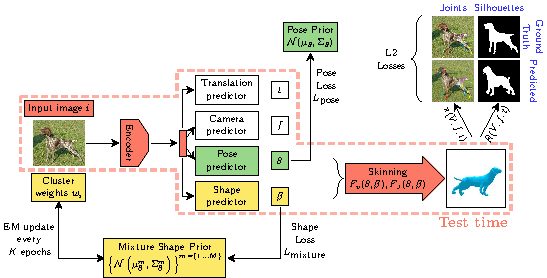
\includegraphics[width=\textwidth]{OllieFigs/system_overview_cr.pdf}
    \caption{Our method consists of (1) a deep CNN encoder which condenses the input image into a feature vector (2) a set of prediction heads which generate SMBLD parameters for shape $\beta$, pose $\theta$, camera focal length $f$ and translation $t$ (3) skinning functions $F_v$ and $F_J$ which construct the mesh from a set of parameters, and (4) loss functions which minimise the error between projected and ground truth joints and silhouettes. Finally, we incorporate a mixture shape prior (5) which regularises the predicted 3D shape and is iteratively updated during training using expectation maximisation. At test time, our system (1) condenses the input image, (2) generates the SMBLD parameters and (3) constructs the mesh.}
    \label{fig:sys_overview_train_sup}
\end{figure*}
    